\section{Couleurs et éclairage}

\begin{frame}{Couleurs et éclairage}
\begin{center}
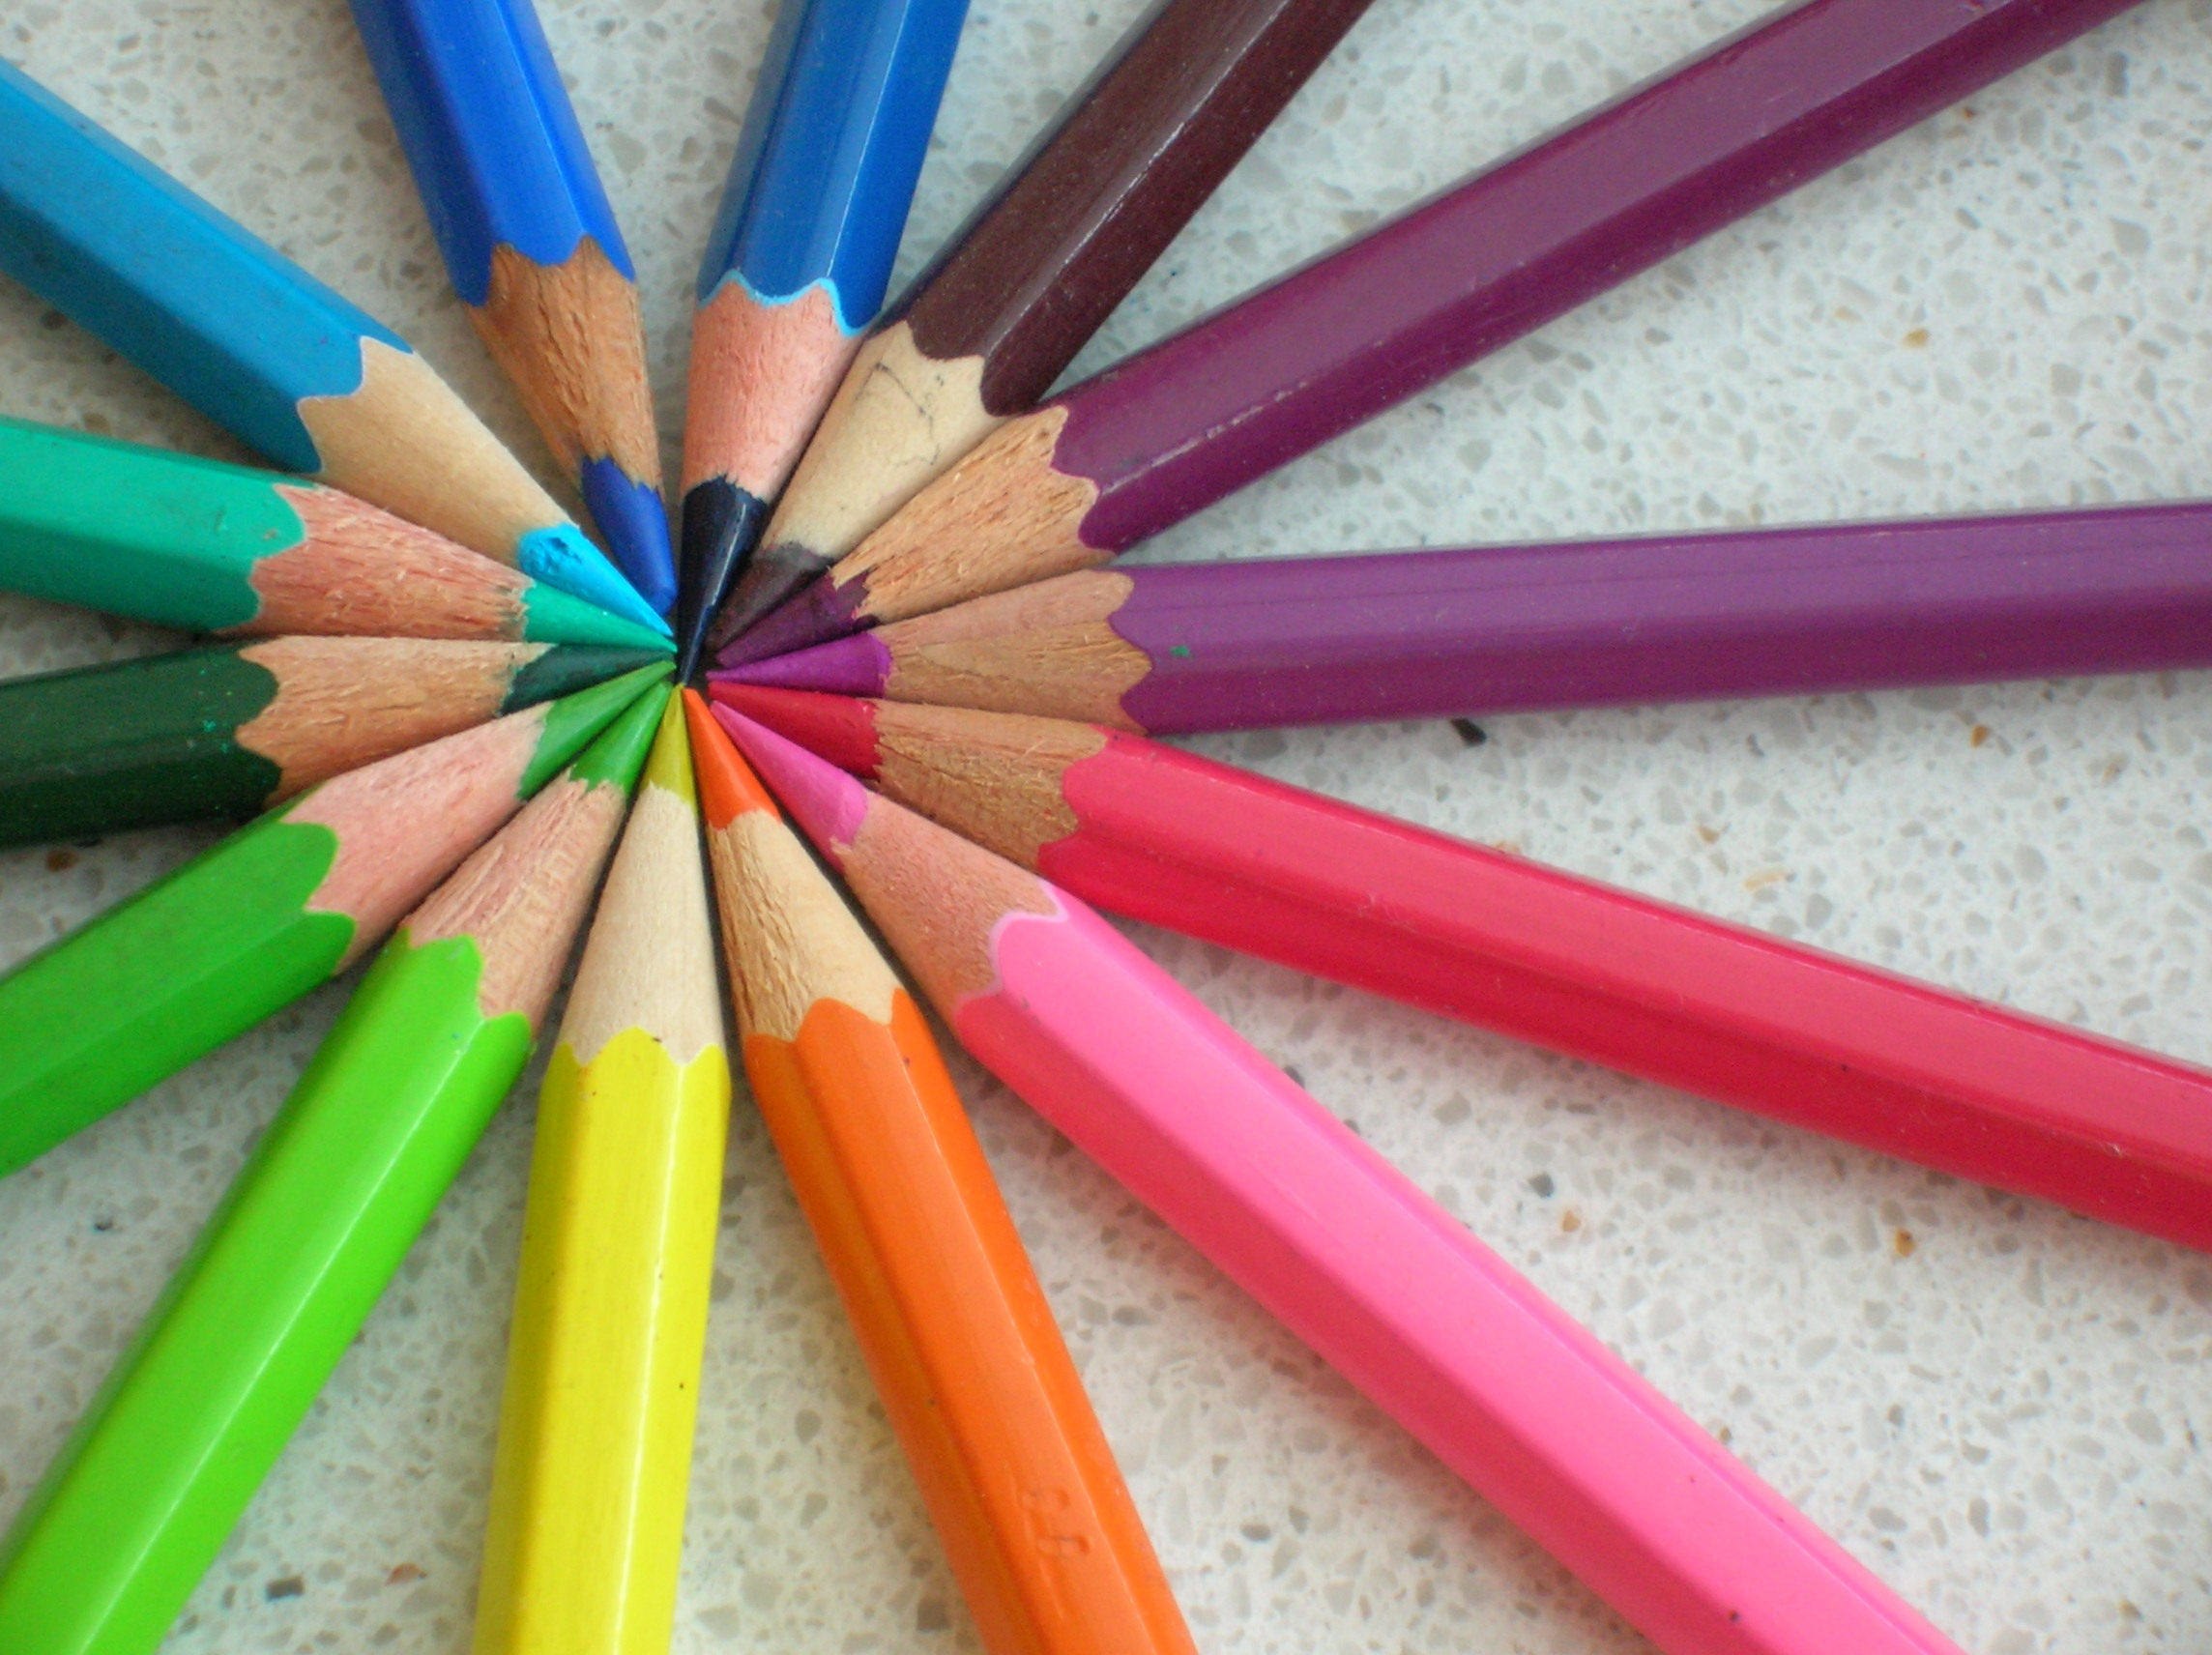
\includegraphics[height=.6\textheight]{figs/Colored_pencils_chevre.jpg}
\end{center}
\end{frame}

\begin{frame}{Lumière}
\begin{center}
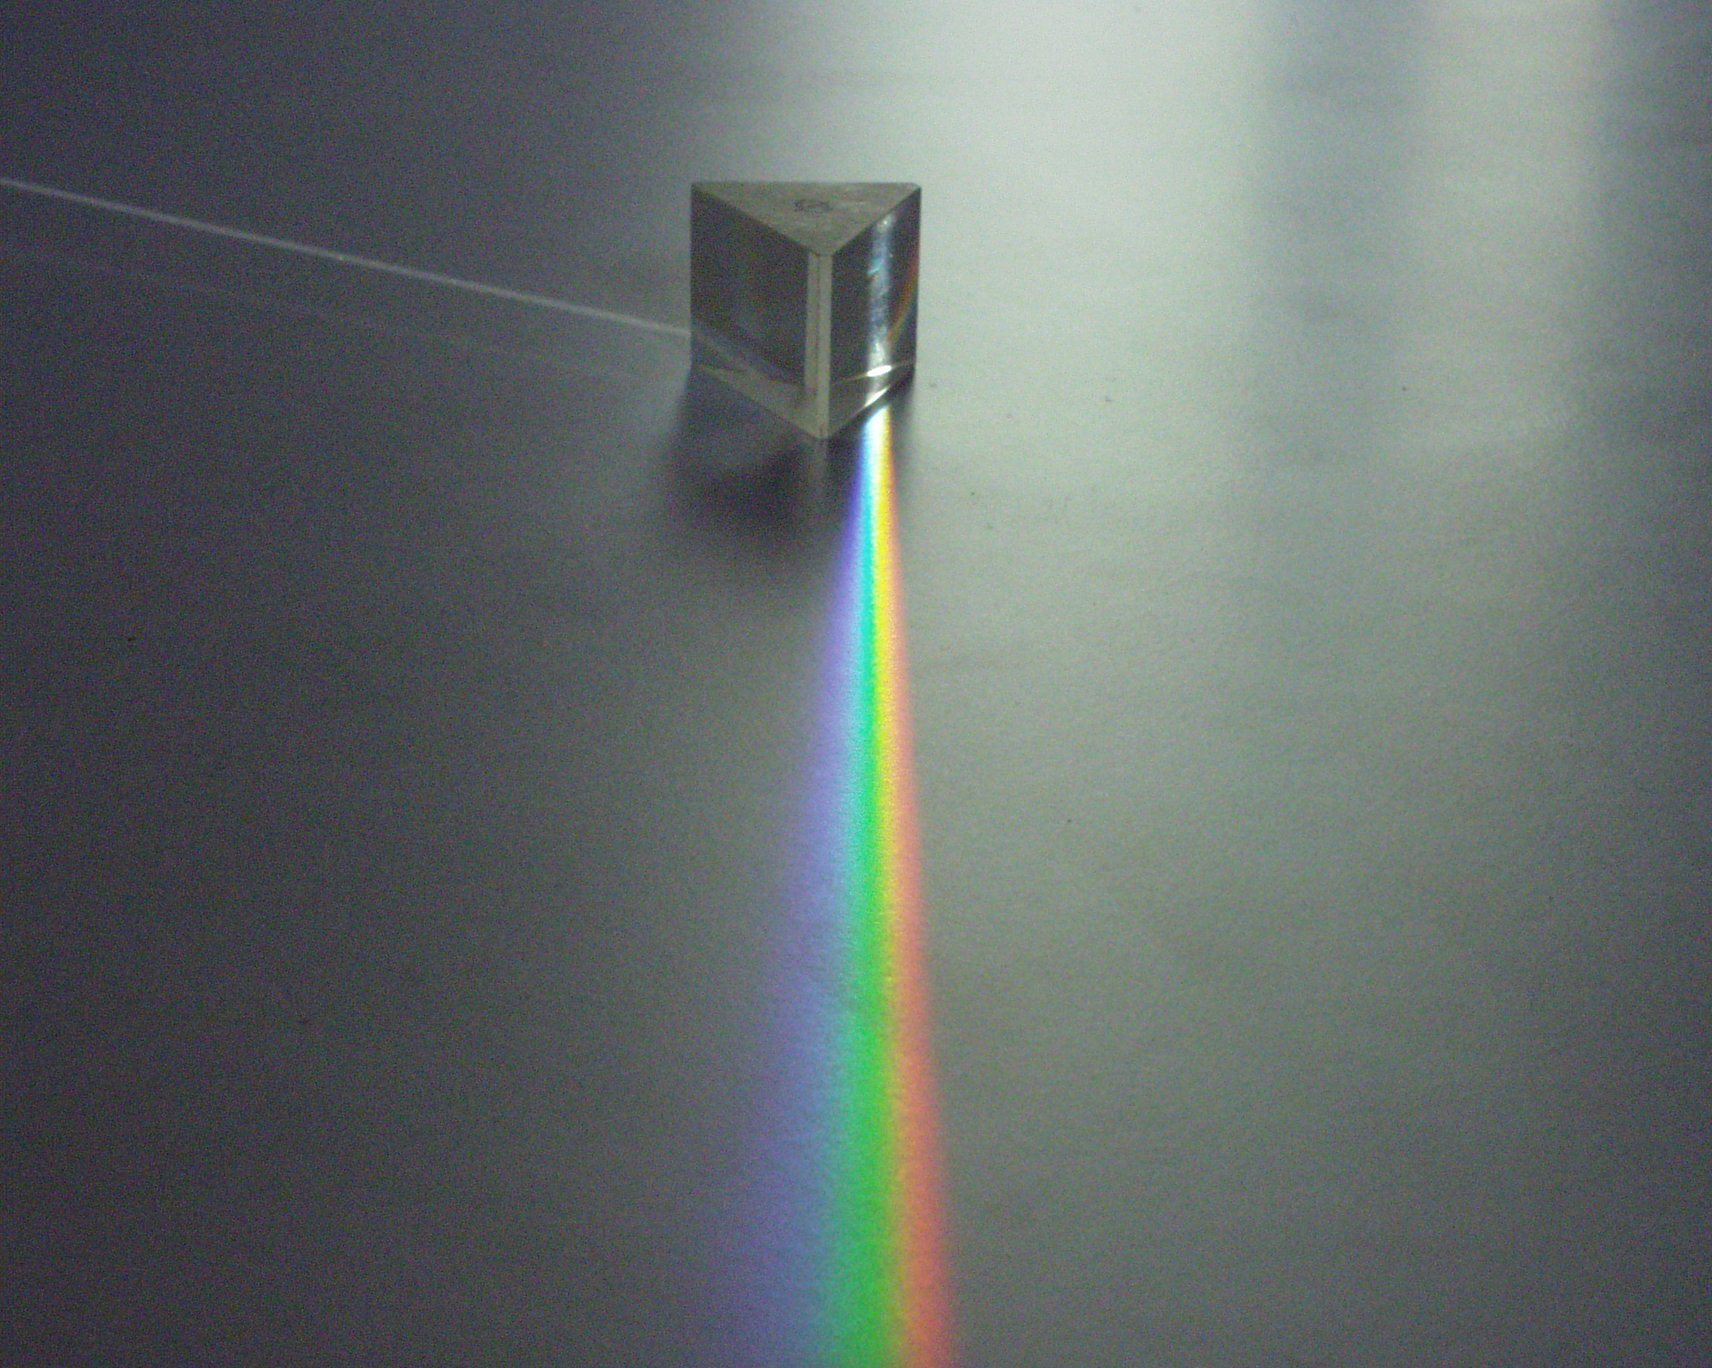
\includegraphics[height=.6\textheight]{figs/prisme.jpg}
\end{center}
\end{frame}

\begin{frame}{Lumière : définition physique}
\begin{columns}
\begin{column}{.6\textwidth}
\begin{itemize}
\item La lumière est caractérisée par son spectre d'absorption
\begin{itemize}
\item La quantité d'énergie pour chaque longueur d'onde
\item Lumière visible : de 380 à 720nm (à peu près)
\begin{itemize}
\item en dessous de 380nm : ultra-violet
\item au dessus de 720nm : infrarouge
\end{itemize}
\end{itemize}
\end{itemize}
\end{column}
\begin{column}{.39\textwidth}
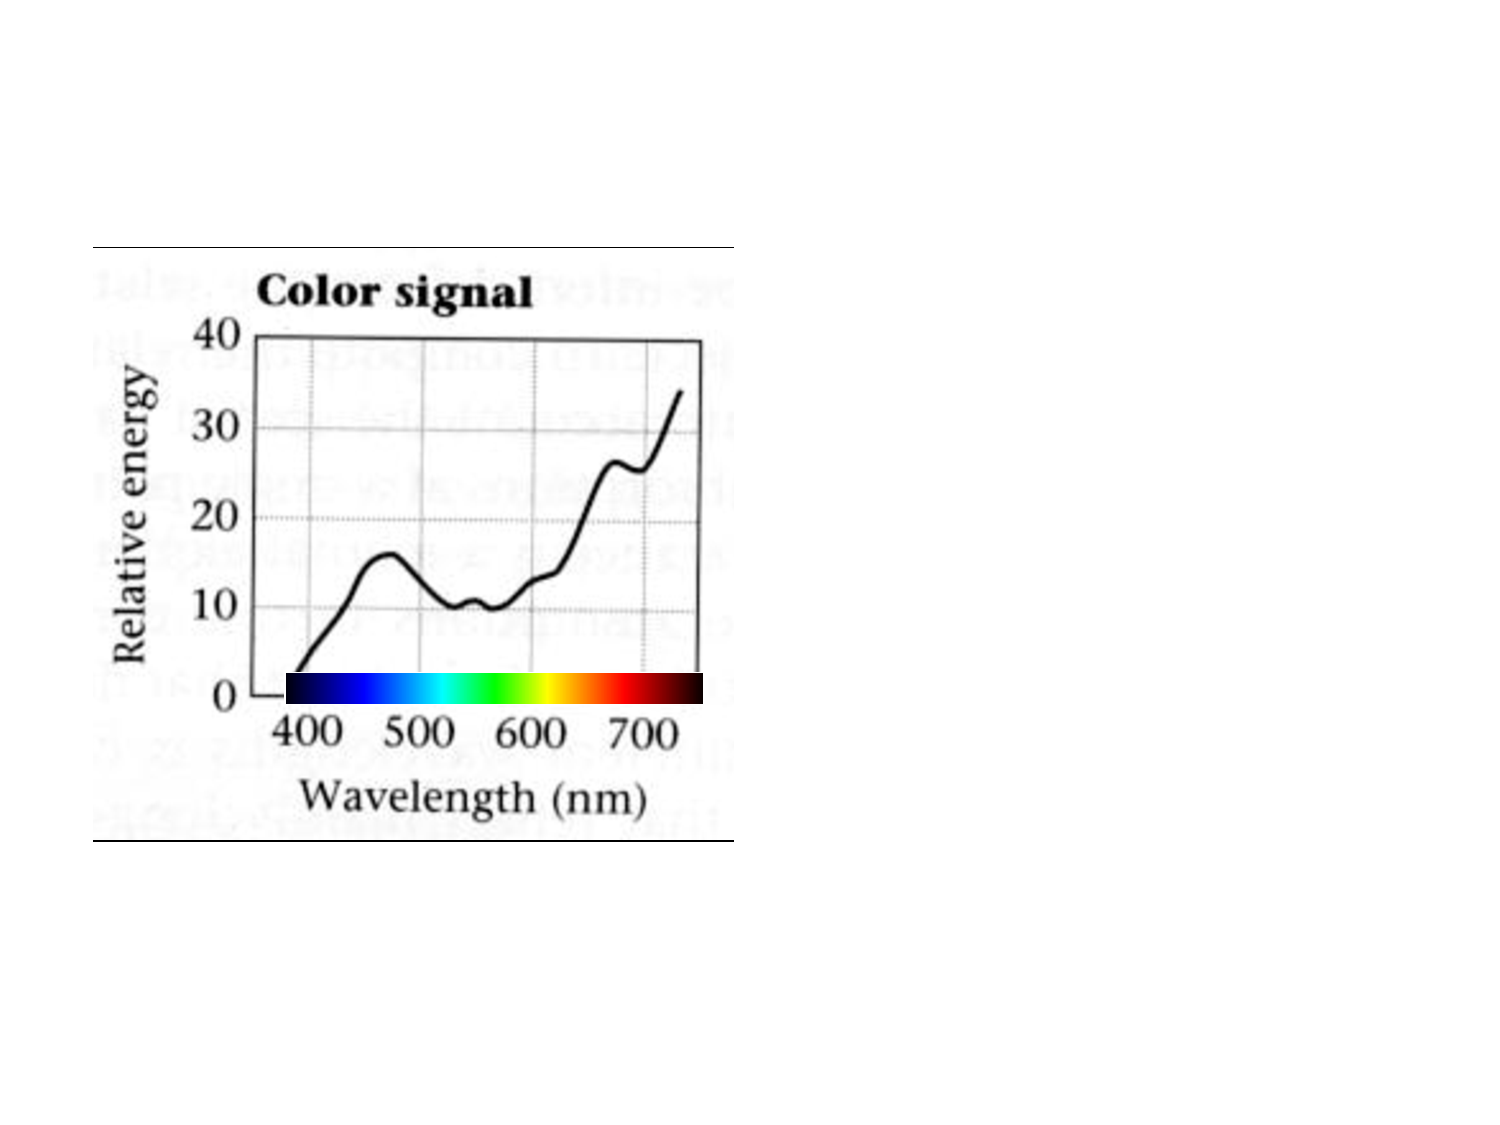
\includegraphics[width=.8\textwidth]{figs/spectre.pdf} \\
\vspace{1cm}
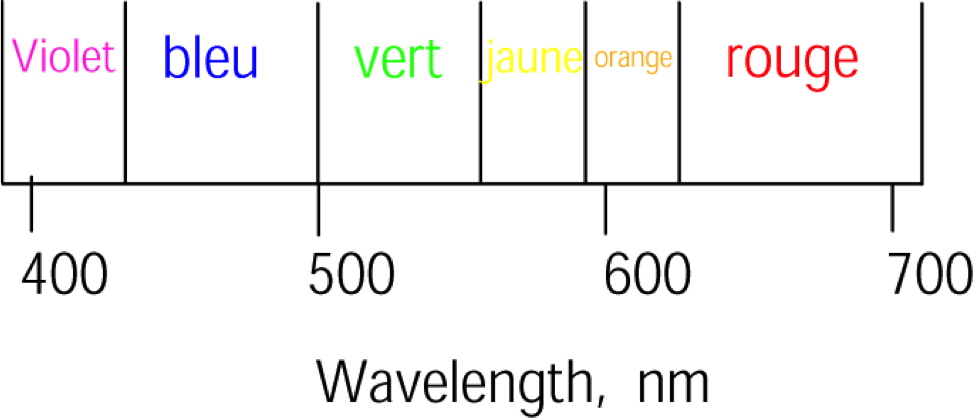
\includegraphics[width=.8\textwidth]{figs/lumsp.png} \\

\end{column}
\end{columns}
\end{frame}

\begin{frame}{Interaction lumière-matière}
\begin{center}
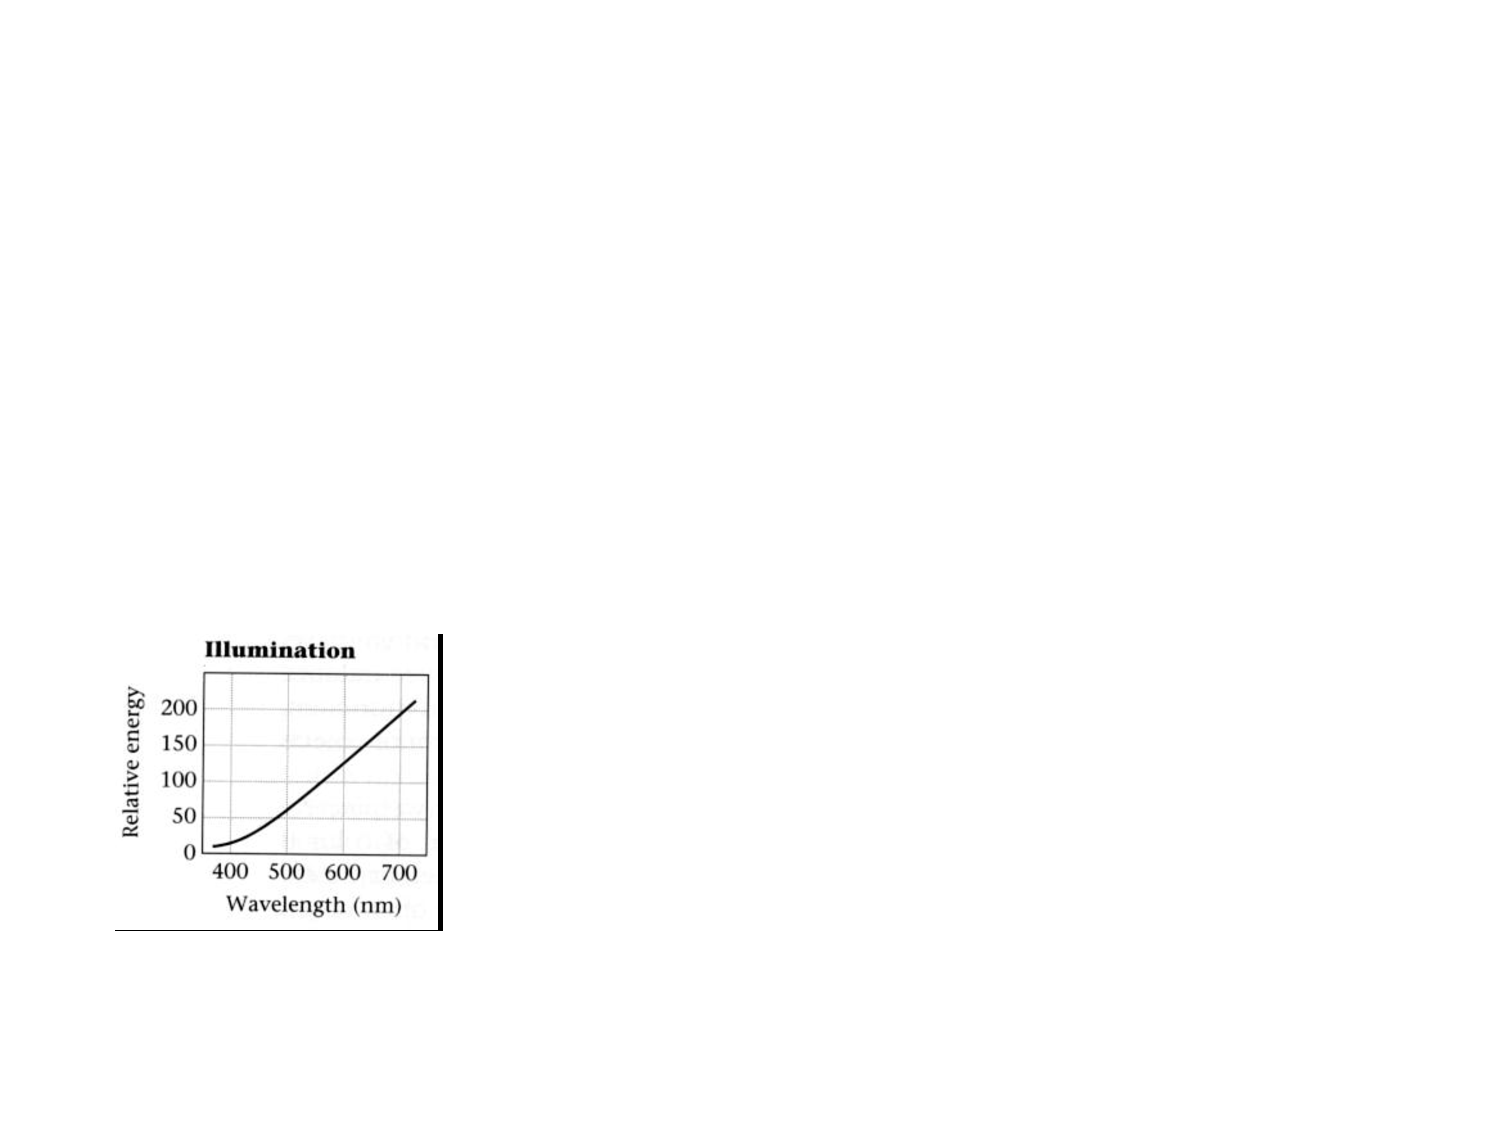
\includegraphics[height=.3\textheight]{figs/lumillum.pdf}
{\Huge .*}
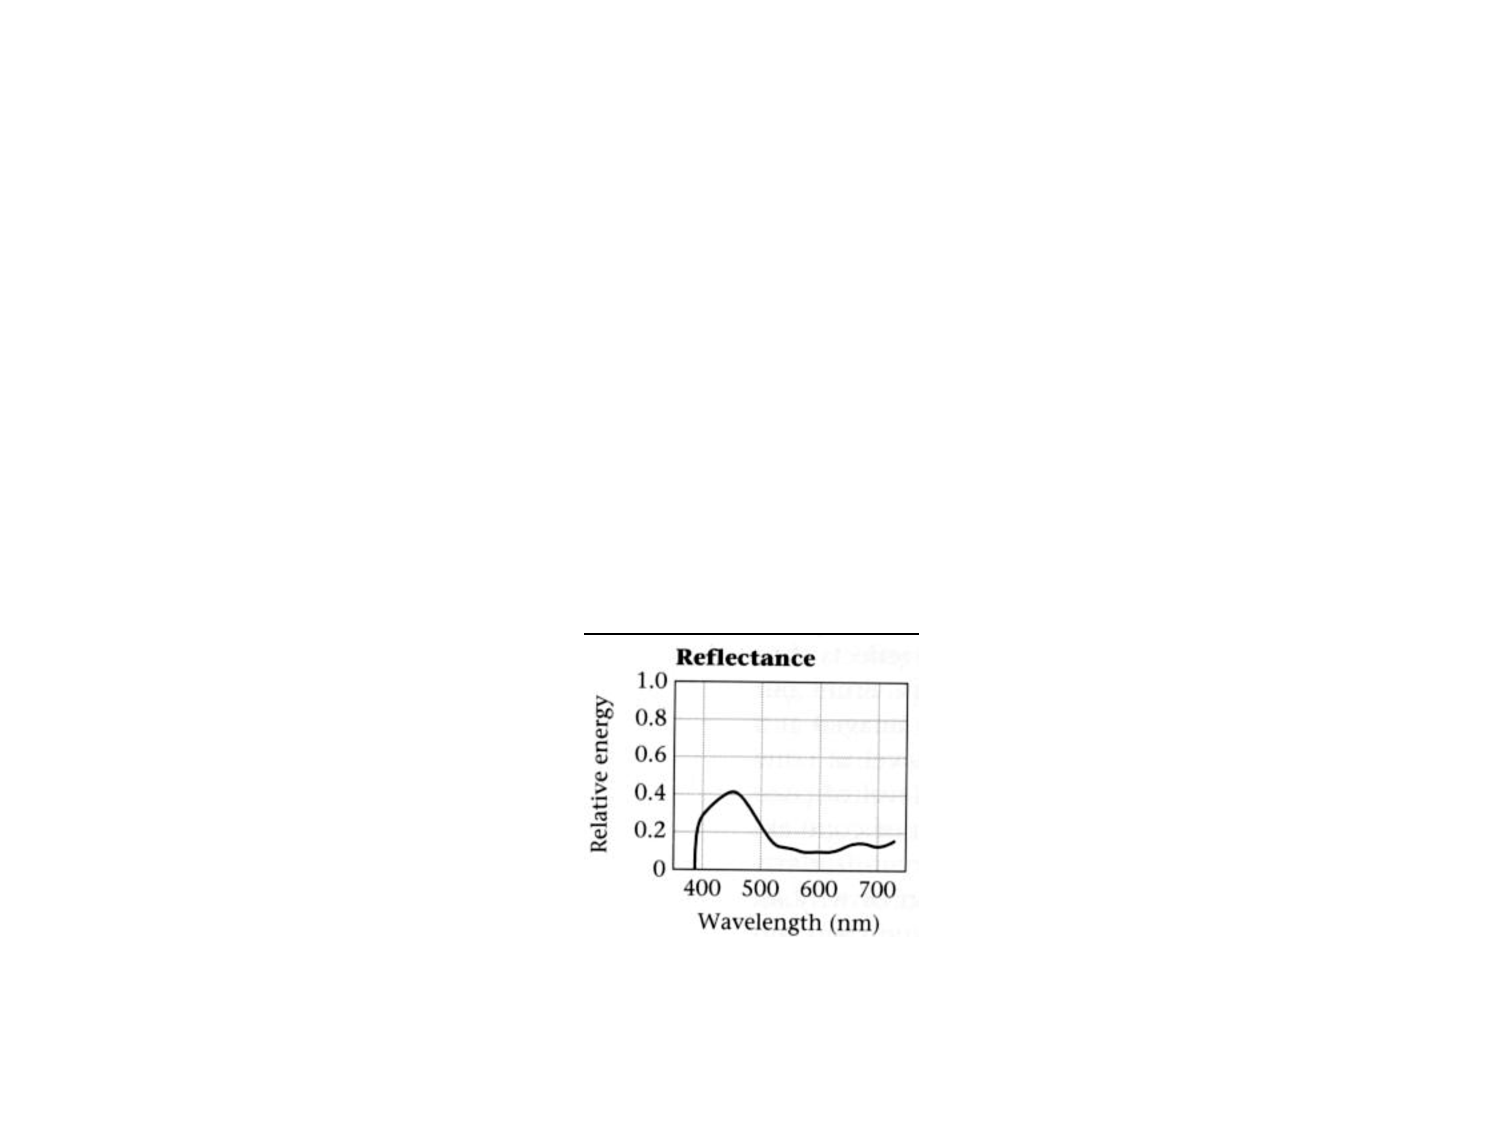
\includegraphics[height=.3\textheight]{figs/lumref.pdf}
{\Huge =}
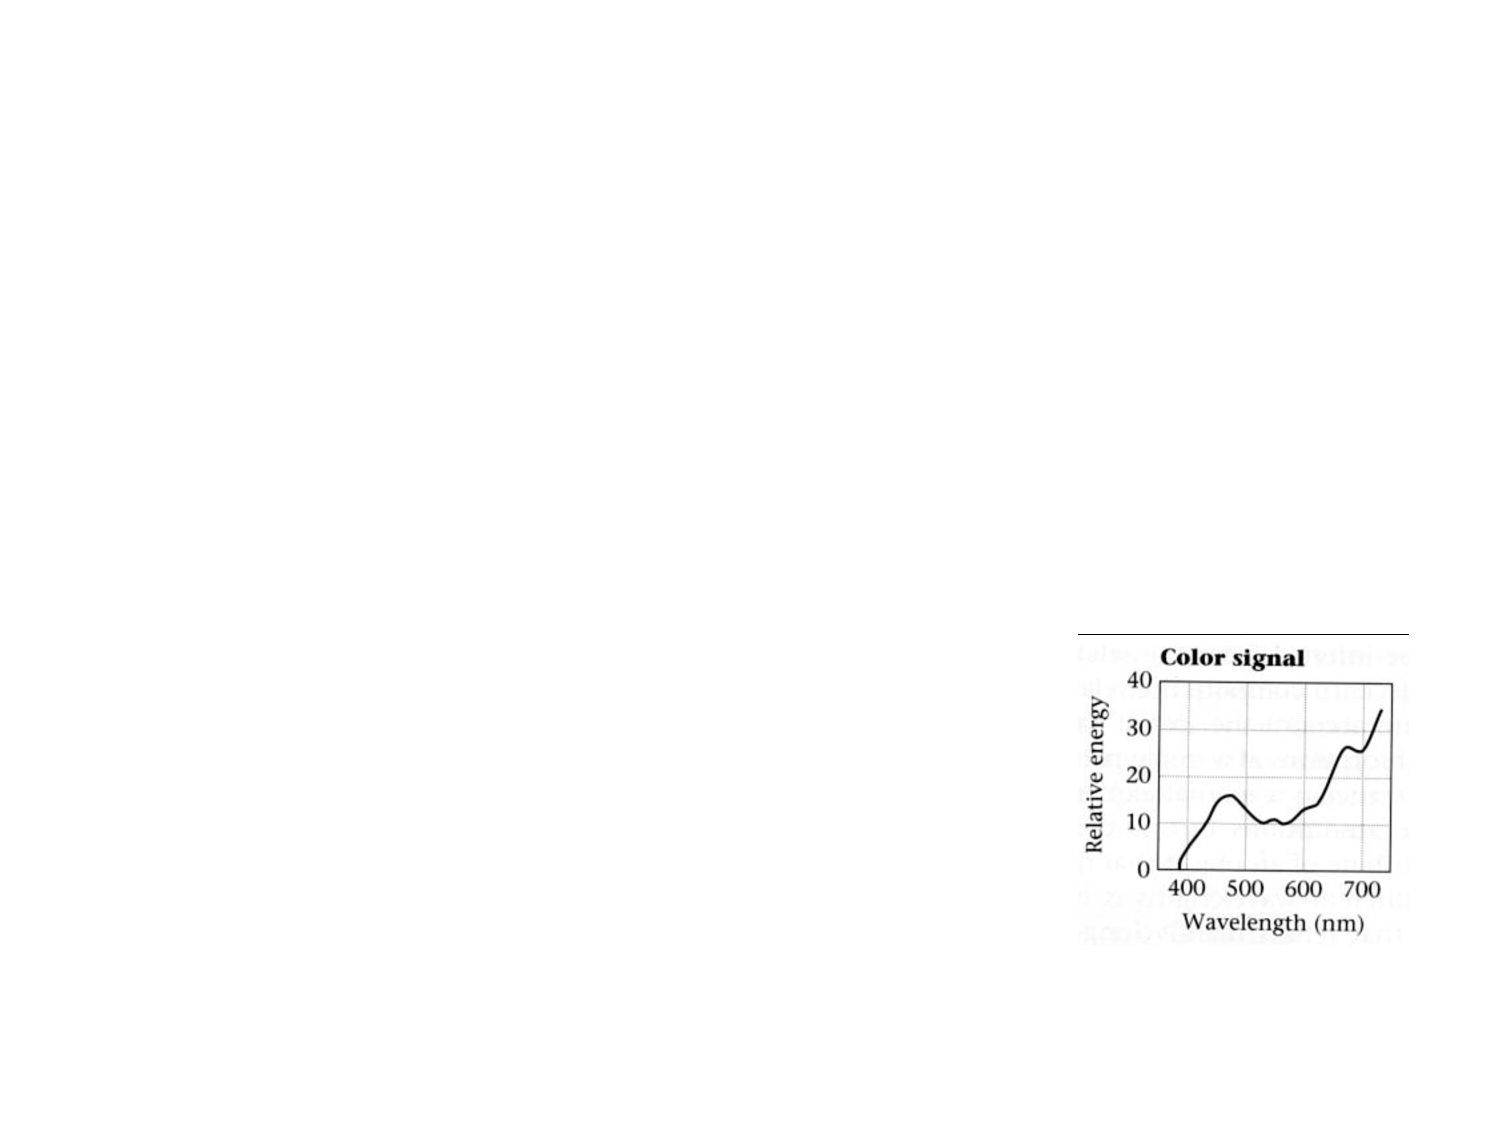
\includegraphics[height=.3\textheight]{figs/lumsig.pdf}

\end{center}
\begin{itemize}
\item La lumière provient :
\begin{itemize}
\item des sources lumineuses
\item de la réflectance des objets
\end{itemize}
\end{itemize}
\end{frame}

\begin{frame}{Lumière : autre définition}
\begin{itemize}
\item Définition basée sur le vocabulaire usuel de la peinture
\item Utilisant le mélange des couleurs
\end{itemize}
\begin{center}
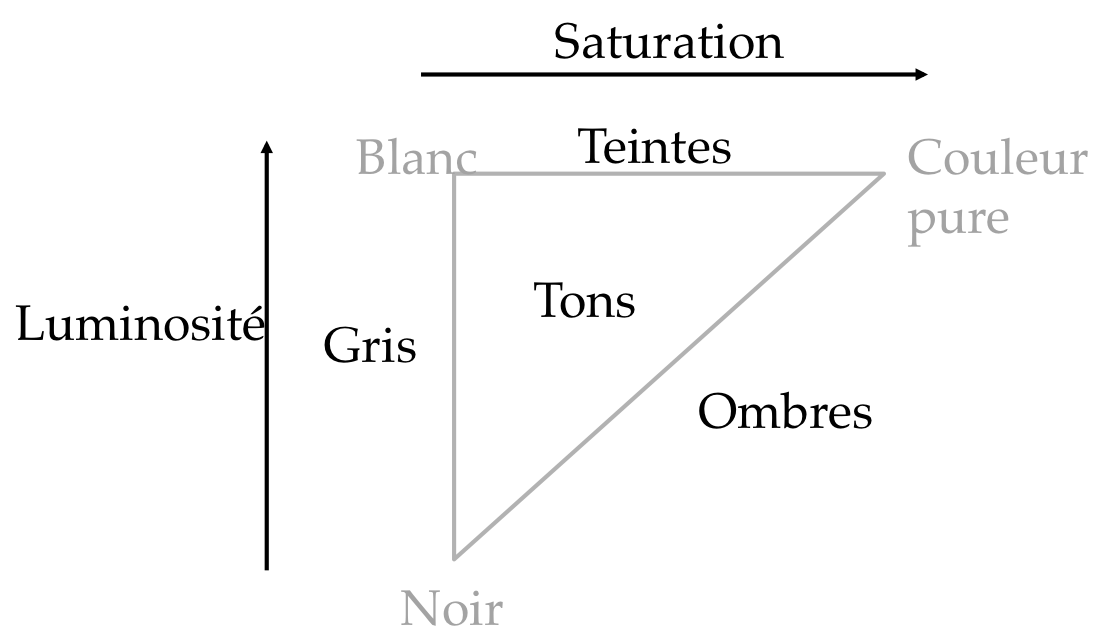
\includegraphics[height=.6\textheight]{figs/lump.png}
\end{center}
\end{frame}

\begin{frame}{Définition spectrale simplifiée}
\begin{center}

\includegraphics[height=.75\textheight]{figs/lumsimpl.png}
\end{center}
\end{frame}

\begin{frame}{De la lumière à la couleur}

\begin{center}
\includegraphics<1>[width=.8\textwidth]{figs/color1.pdf}
\includegraphics<2>[width=.8\textwidth]{figs/color2.pdf}
\includegraphics<3>[width=.8\textwidth]{figs/color3.pdf}

\end{center}
\begin{itemize}
\item On abordera le système visuel humain dans le cours FONRV
\end{itemize}
\end{frame}

\begin{frame}{Réponse des cônes}
\begin{center}
\includegraphics<1>[height=.8\textheight]{figs/cone.pdf}
\includegraphics<2>[height=.8\textheight]{figs/conecomplet.pdf}
\end{center}
\end{frame}

\begin{frame}{Un cône ne perçoit pas vraiment les couleurs !}
\begin{itemize}
\item Longueur d'onde différente, intensité différente
\item Même réponse
\item<2> Mais réponse différence pour les différents types de cônes
\end{itemize}
\begin{center}
\includegraphics<1>[height=.6\textheight]{figs/conecl.pdf}
\includegraphics<2>[height=.6\textheight]{figs/conecl2.pdf}
\end{center}

\end{frame}

\begin{frame}{Théorie tri-chromatique de von Helmholtz, 1859}
\begin{itemize}
\item Les couleurs sont définis comme des ratios de réponses entre les différents types de cônes
\end{itemize}
\begin{center}
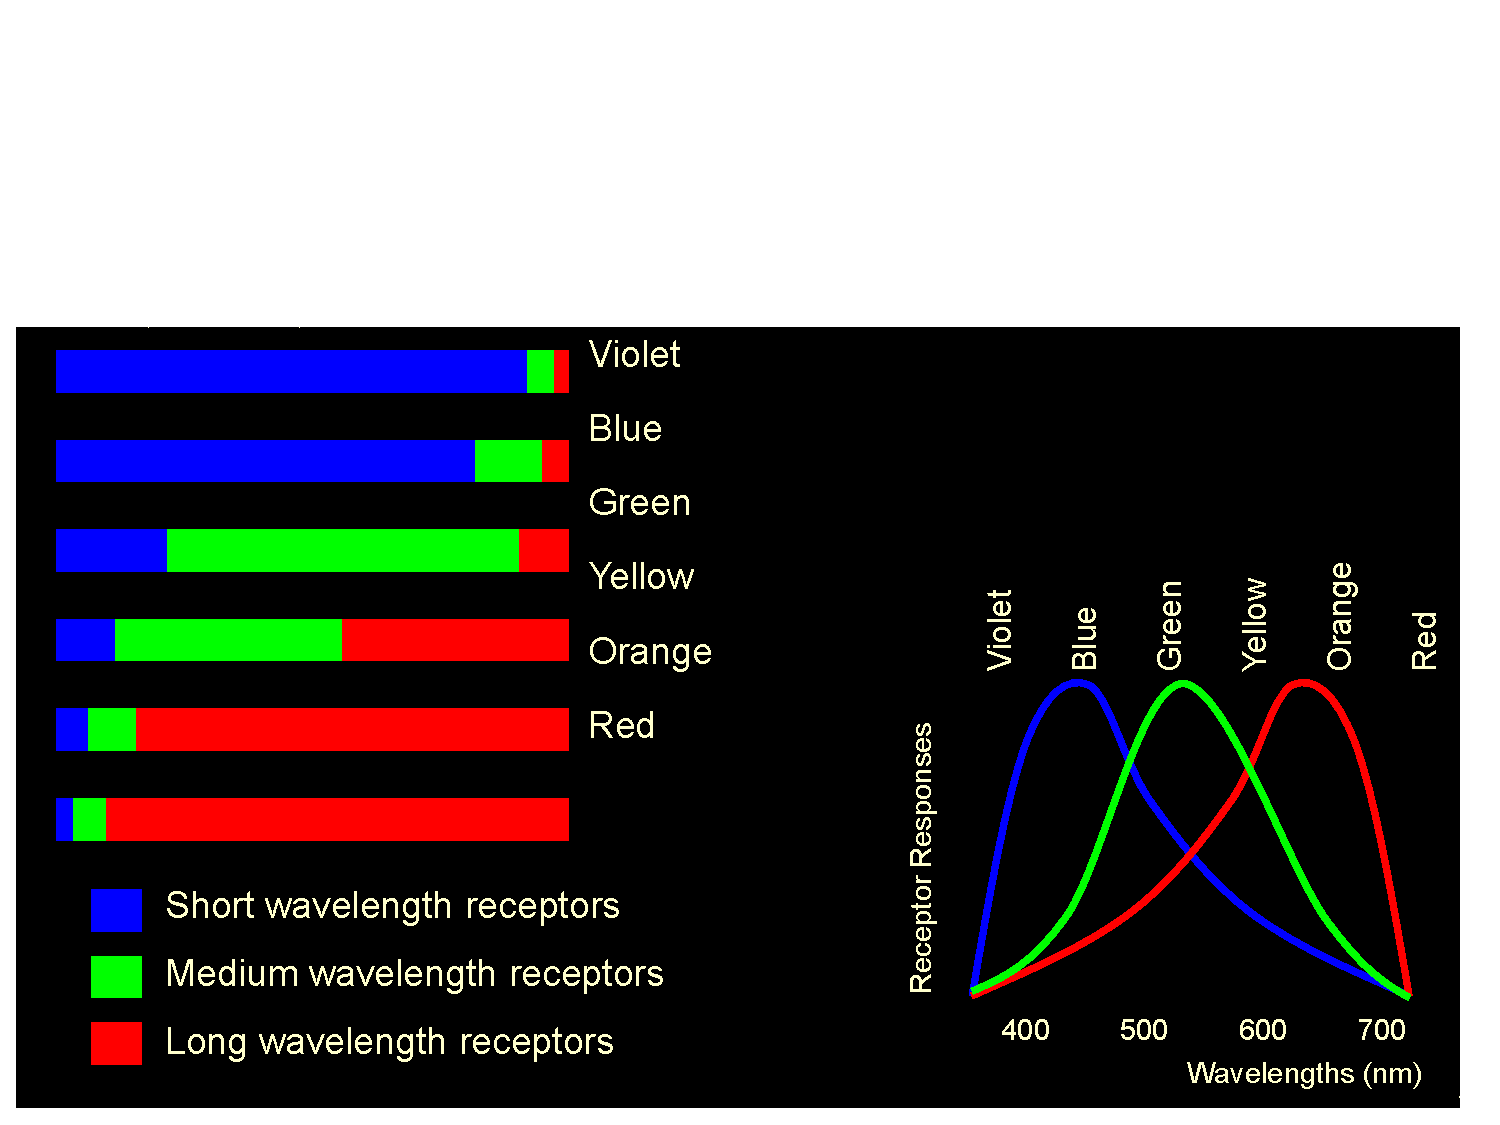
\includegraphics[height=.7\textheight]{figs/couleurs}
\end{center}
\end{frame}

\subsection{Représentation des couleurs}

\begin{frame}{Représentation des couleurs}
\begin{itemize}
\item La représentation spectrale est trop riche
\begin{itemize}
\item Par rapport à la vision humaine
\item En coût mémoire (et de calcul)
\end{itemize}
\item La vision humaine n'a que 3 fonctions de base
\item On doit pouvoir en tirer une représentation compacte
\begin{itemize}
\item A partir de couleurs primaires
\end{itemize}
\end{itemize}
\end{frame}

\begin{frame}{Lois de Grassmman}
\begin{enumerate}
\item toute couleur peut être représentée au moyen d'au plus 3 couleurs primaires

\item le système visuel ne sait pas identifier les couleurs primaires lors du rendu

\item 4 couleurs sont toujours liées linéairement

\item l'espace des couleurs est continu

\begin{center}
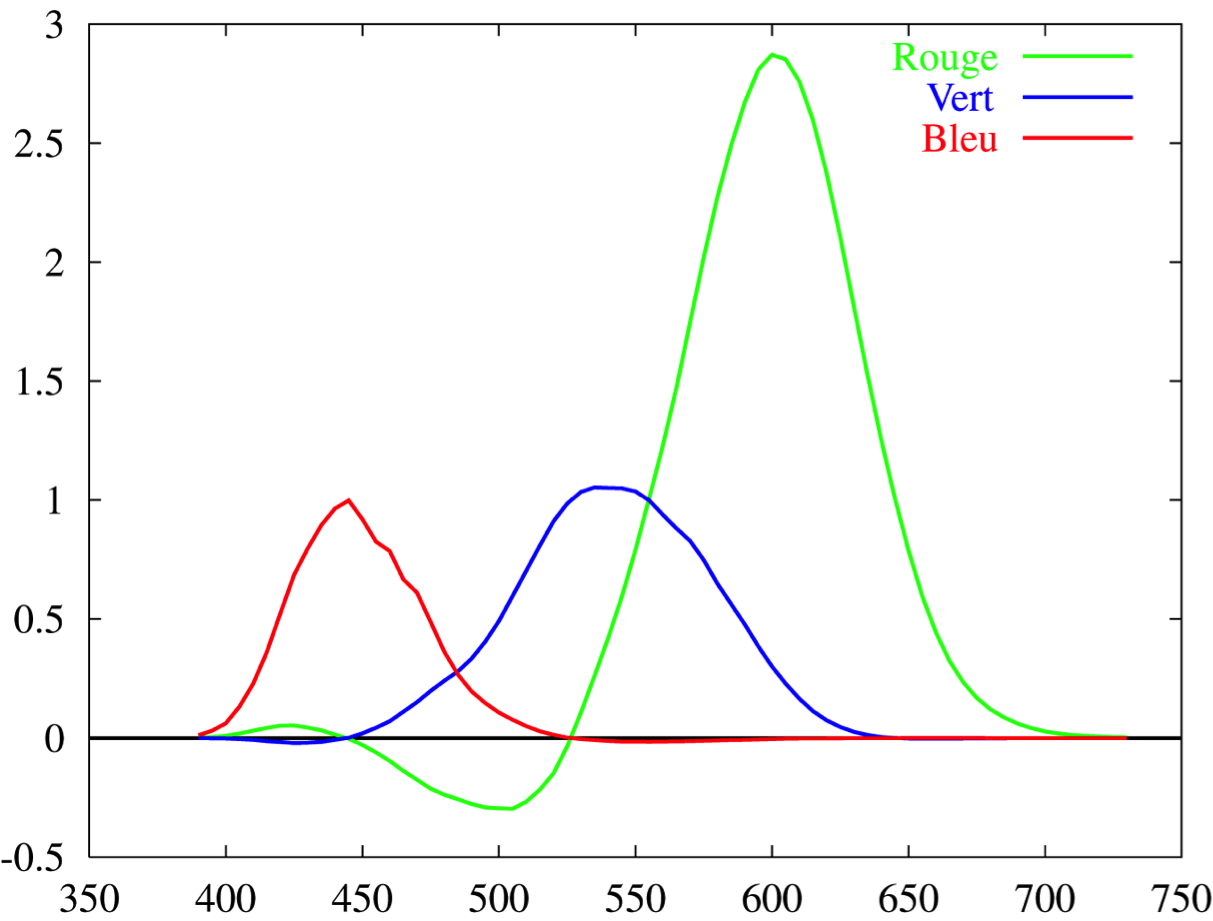
\includegraphics[height=.4\textheight]{figs/rgbsp.png}
\end{center}
\end{enumerate}
\end{frame}

\begin{frame}{CIE XYZ}
\begin{itemize}
\item Norme datant de 1931
\item Nouvelle fonction de base à partir de la courbe précédente
\begin{itemize}
\item 3 couleurs monochromatiques
\item Quelques astuces pour arriver à des valeurs positives
\end{itemize}
\end{itemize}
\begin{center}
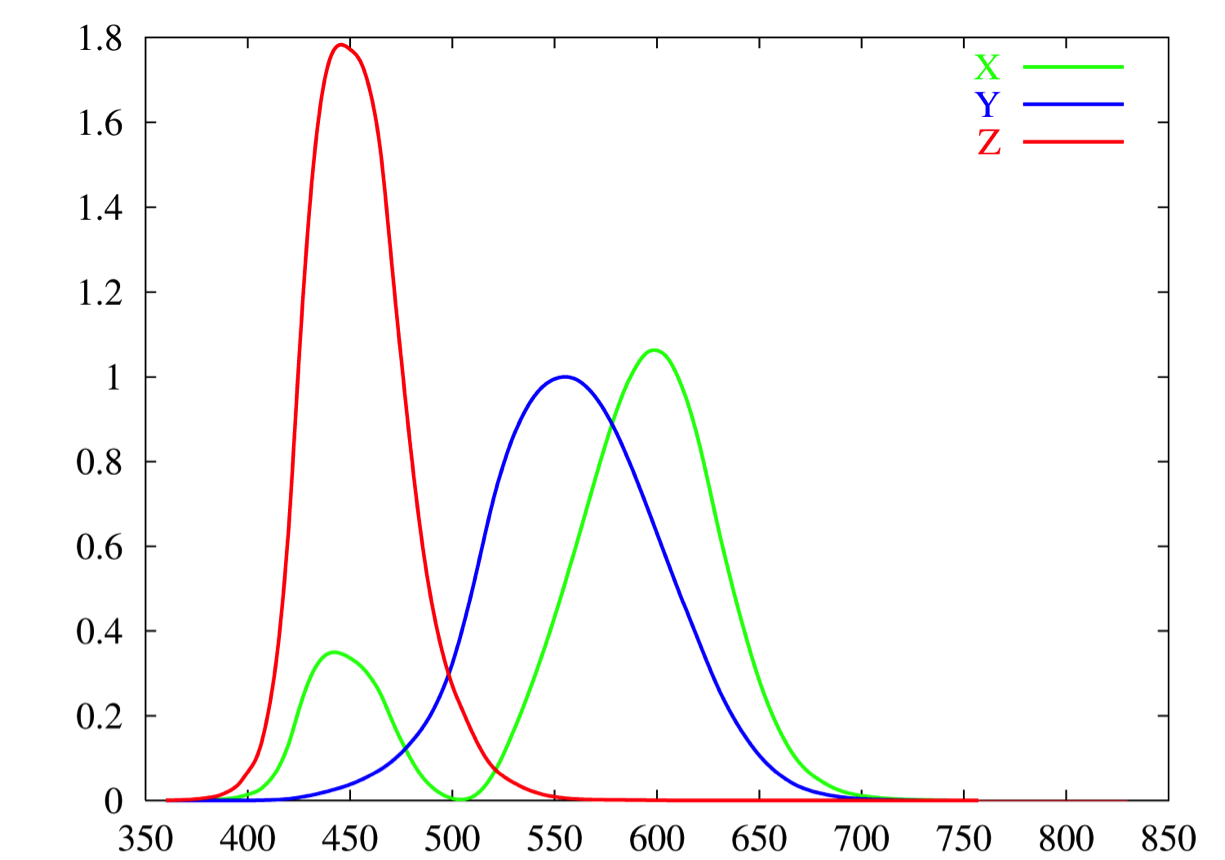
\includegraphics[height=.4\textheight]{figs/cie-xyz.png}
\end{center}
\end{frame}

\begin{frame}{CIE XYZ}
\begin{itemize}
\item Y = luminance (perçue par la vision humaine)
\item X,Y,Z : représente toutes les couleurs
\item Conversion vers R,B,G linéaire
\begin{itemize}
\item Simple multiplication par une matrice 3x3
\end{itemize}
\item Manque de \textit{sens}
\begin{itemize}
\item Le même rouge en plus saturé
\end{itemize}
\end{itemize}
\begin{center}
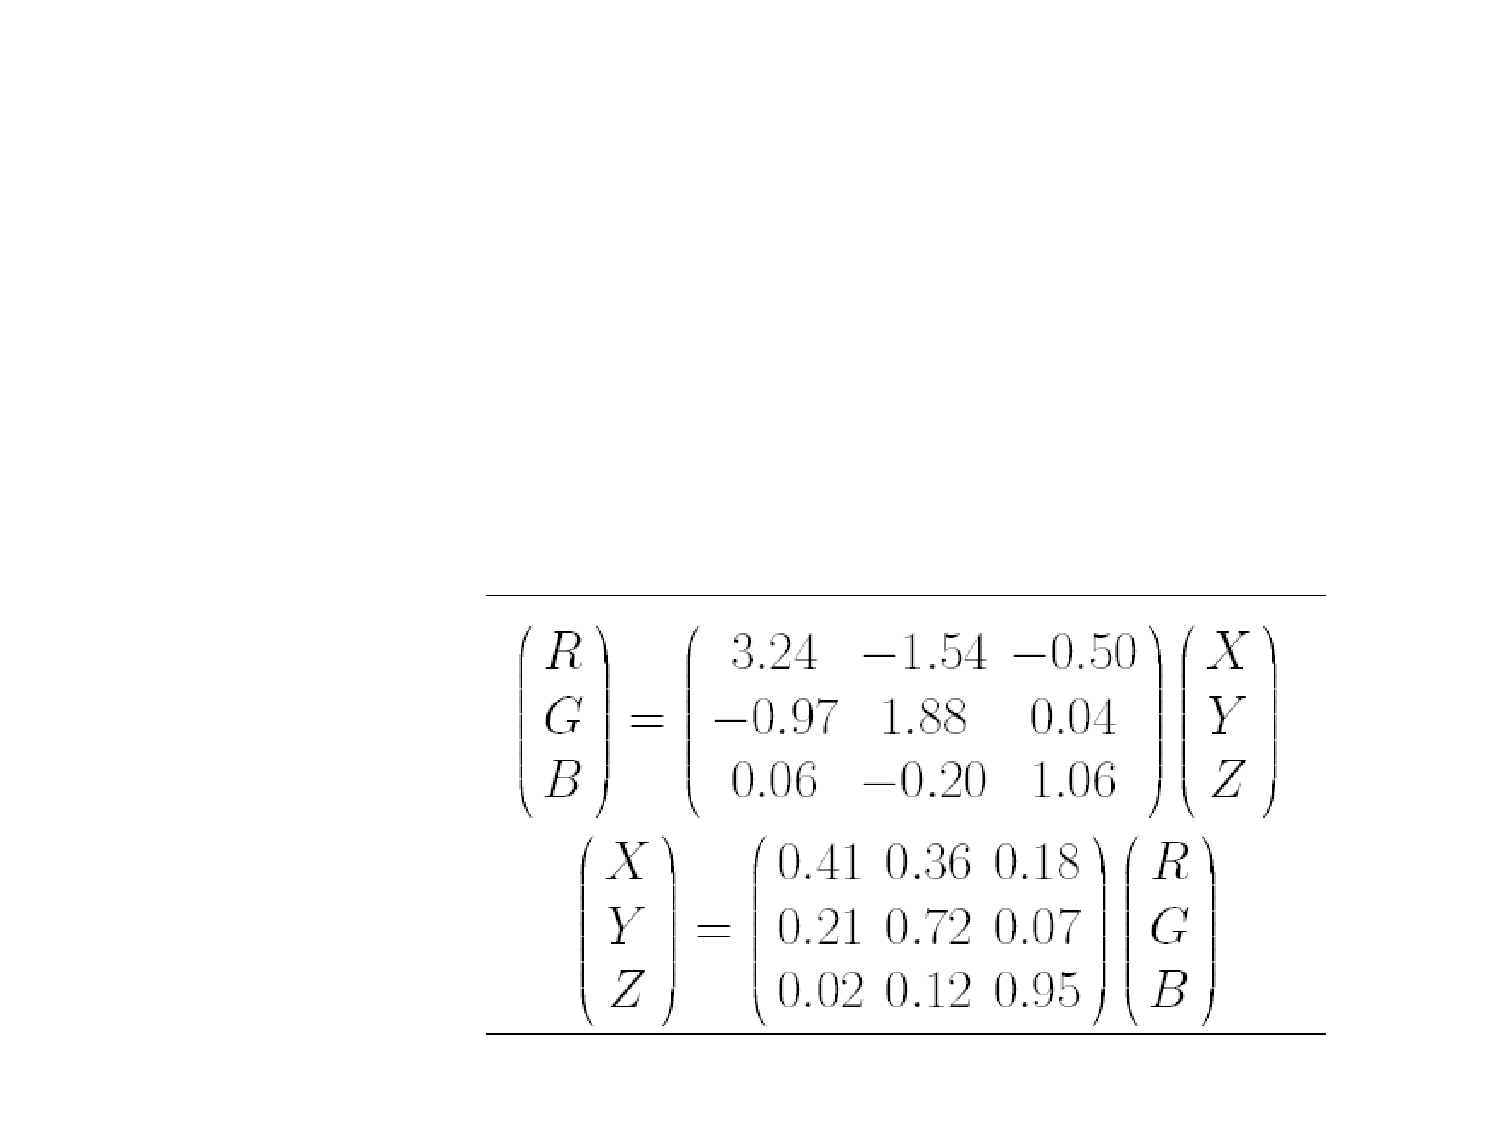
\includegraphics[height=.4\textheight]{figs/rgbxyz}
\end{center}
\end{frame}

\begin{frame}{Chromaticité}
\begin{itemize}
\item On introduit $x,y$
$$ x = \frac{X}{X+Y+Z}, y=\frac{Y}{X+Y+Z}$$
\item Diagramme de chromaticité
\end{itemize}
\begin{center}
\includegraphics<1>[height=.5\textheight]{figs/chromaticite.png}
\includegraphics<2>[height=.5\textheight]{figs/chromaticite2.png}
\includegraphics<3>[height=.5\textheight]{figs/chromaticite3.png}

\end{center}

\end{frame}

\begin{frame}{Couleurs représentables}
\begin{itemize}
\item Plus intéressant :
\begin{itemize}
\item<1> Quelles couleurs savent reproduire nos dispositifs habituels ?
\item<2> Quelles couleurs savent distinguer nos yeux ?
\end{itemize}
\end{itemize}
\begin{center}
\includegraphics<1>[height=.5\textheight]{figs/chroma4.png}
\includegraphics<2>[height=.5\textheight]{figs/chroma5.png}

\end{center}
\end{frame}

\begin{frame}{Quelques systèmes de représentation des couleurs}
\begin{itemize}
\item Systèmes basés sur l'outil d'affichage
\begin{itemize}
\item RGB
\item CMYK
\item Yuv
\end{itemize}
\item Systèmes basés sur l'IHM
\begin{itemize}
\item HSV
\end{itemize}
\item Conversion possibles ? Quels outils ?
\end{itemize}
\end{frame}

\begin{frame}{Le système RGB}
\begin{itemize}
\item Toute couleur s'exprime comme une combinaison linéaire additive de rouge, vert et bleu
\item Utilisé quasiment partout
\item Système \textbf{additif}
\end{itemize}
\begin{center}
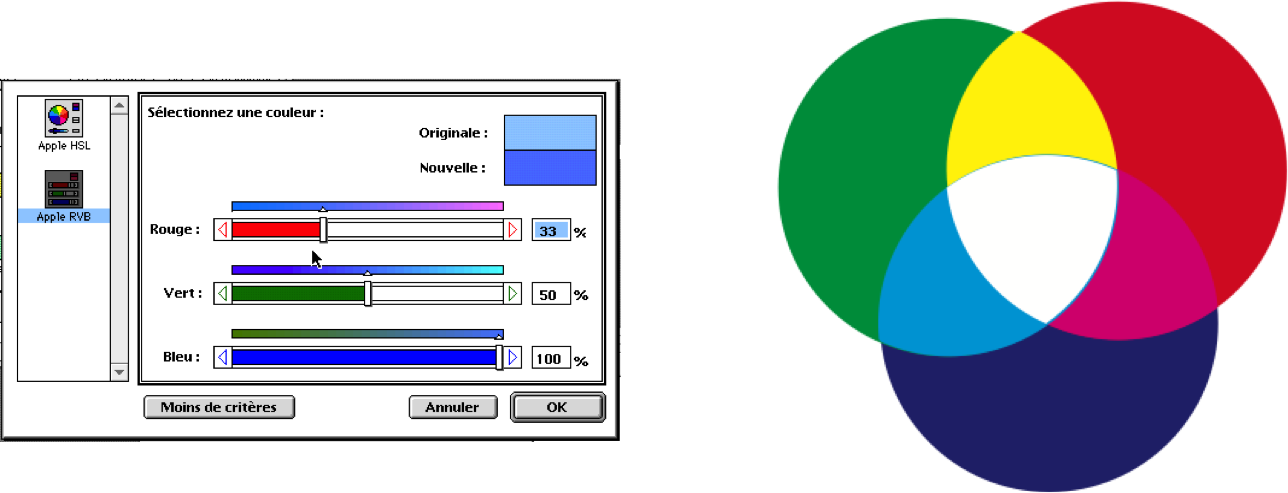
\includegraphics[height=.5\textheight]{figs/rgb.png}

\end{center}
\end{frame}

\begin{frame}{Le système CMY}
\begin{itemize}
\item Système \textbf{soustractif} utilisé par les imprimantes couleur
\item En théorie : $C=1-R$, $M=1-G$, $Y=1-B$
\item En pratique :
\begin{itemize}
\item Conversion non linéaire
\item Contraintes physiques : ordre des couches d'encre, réaction du papier...
\end{itemize}
\end{itemize}
\begin{center}
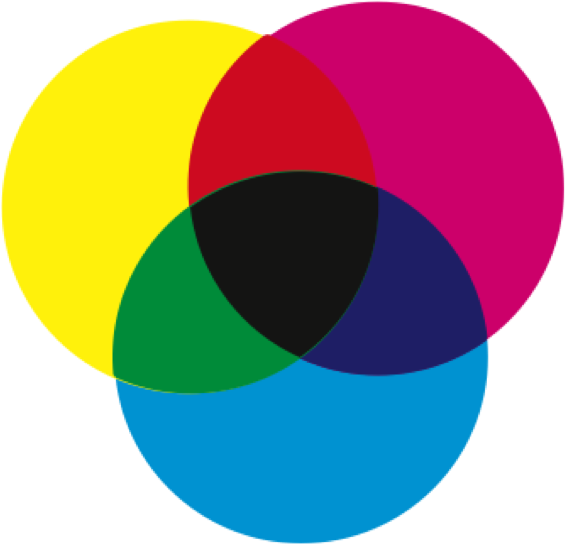
\includegraphics[height=.5\textheight]{figs/cmyk.png}

\end{center}
\end{frame}

\begin{frame}{Le système CMYK}
\begin{itemize}
\item Même chose que CMY avec K (blacK)
\item Mesure d'économie : l'encre noire est moins chère
\item Par exemple : $K=min(C,M,Y)$, $C=C-K$, $M=M-K$, $Y=Y-K$
\item Là encore, purement théorique : le noir ne se mélange pas si bien aux autres couleurs
\end{itemize}
\end{frame}

\begin{frame}{Fonctions de base de type Y}
\begin{itemize}
\item YIQ, Yuv, YCbCr...
\item Utilisés pour la vidéo couleur (analogique)
\begin{itemize}
\item $Y$ : luminance (grande bande passante)
$$Y = LumaRed*R + LumaGreen*G + LumaBlue*B$$
\item $Cb$, $Cr$ : chromaticité (faible bande passante)
$$Cb = (B-Y)/(2-2*LumaBlue)$$
\end{itemize}
\item Une TV noir et blanc ne récupère et n'affiche que $Y$
\item YUV = PAL, YIQ =NTSC
\item Intéressant pour le traitement et la compression d'images !
\end{itemize}
\end{frame}

\begin{frame}{Le système HSV}
\begin{itemize}
\item Hue (teinte), Saturation, Value
\item Se veut intuitif (cf. définition du peintre)
\end{itemize}
\begin{center}
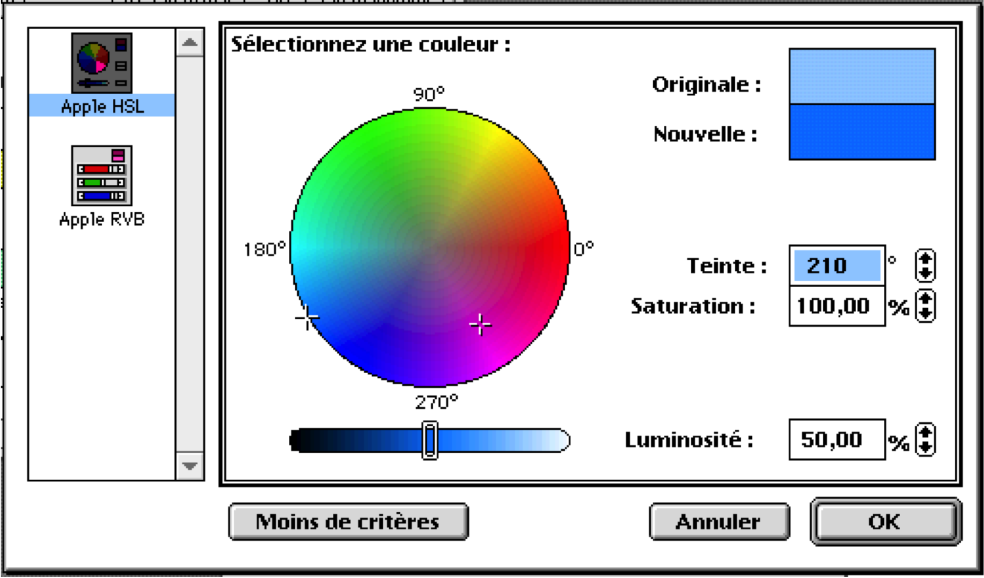
\includegraphics[height=.5\textheight]{figs/hsv.png}

\end{center}
\end{frame}

\begin{frame}[fragile]
\frametitle{Conversion}
\begin{lstlisting}[language=C++]
max = max(R,G,B);
min = min(R,G,B);
V = max;
S = (max-min)/max;
delta = max-min;
if (max ==R) {
  H = (G-B)/delta;
}
else if (max == G) {
  H = 2+(B-R)/delta
}
else if (max == B) {
  H = 4+(R-G)/delta
}
H *= 60;
if (H <0) {
  H += 360;
}
\end{lstlisting}
\end{frame}

\begin{frame}{HSL - HSV - RGB}
\begin{center}
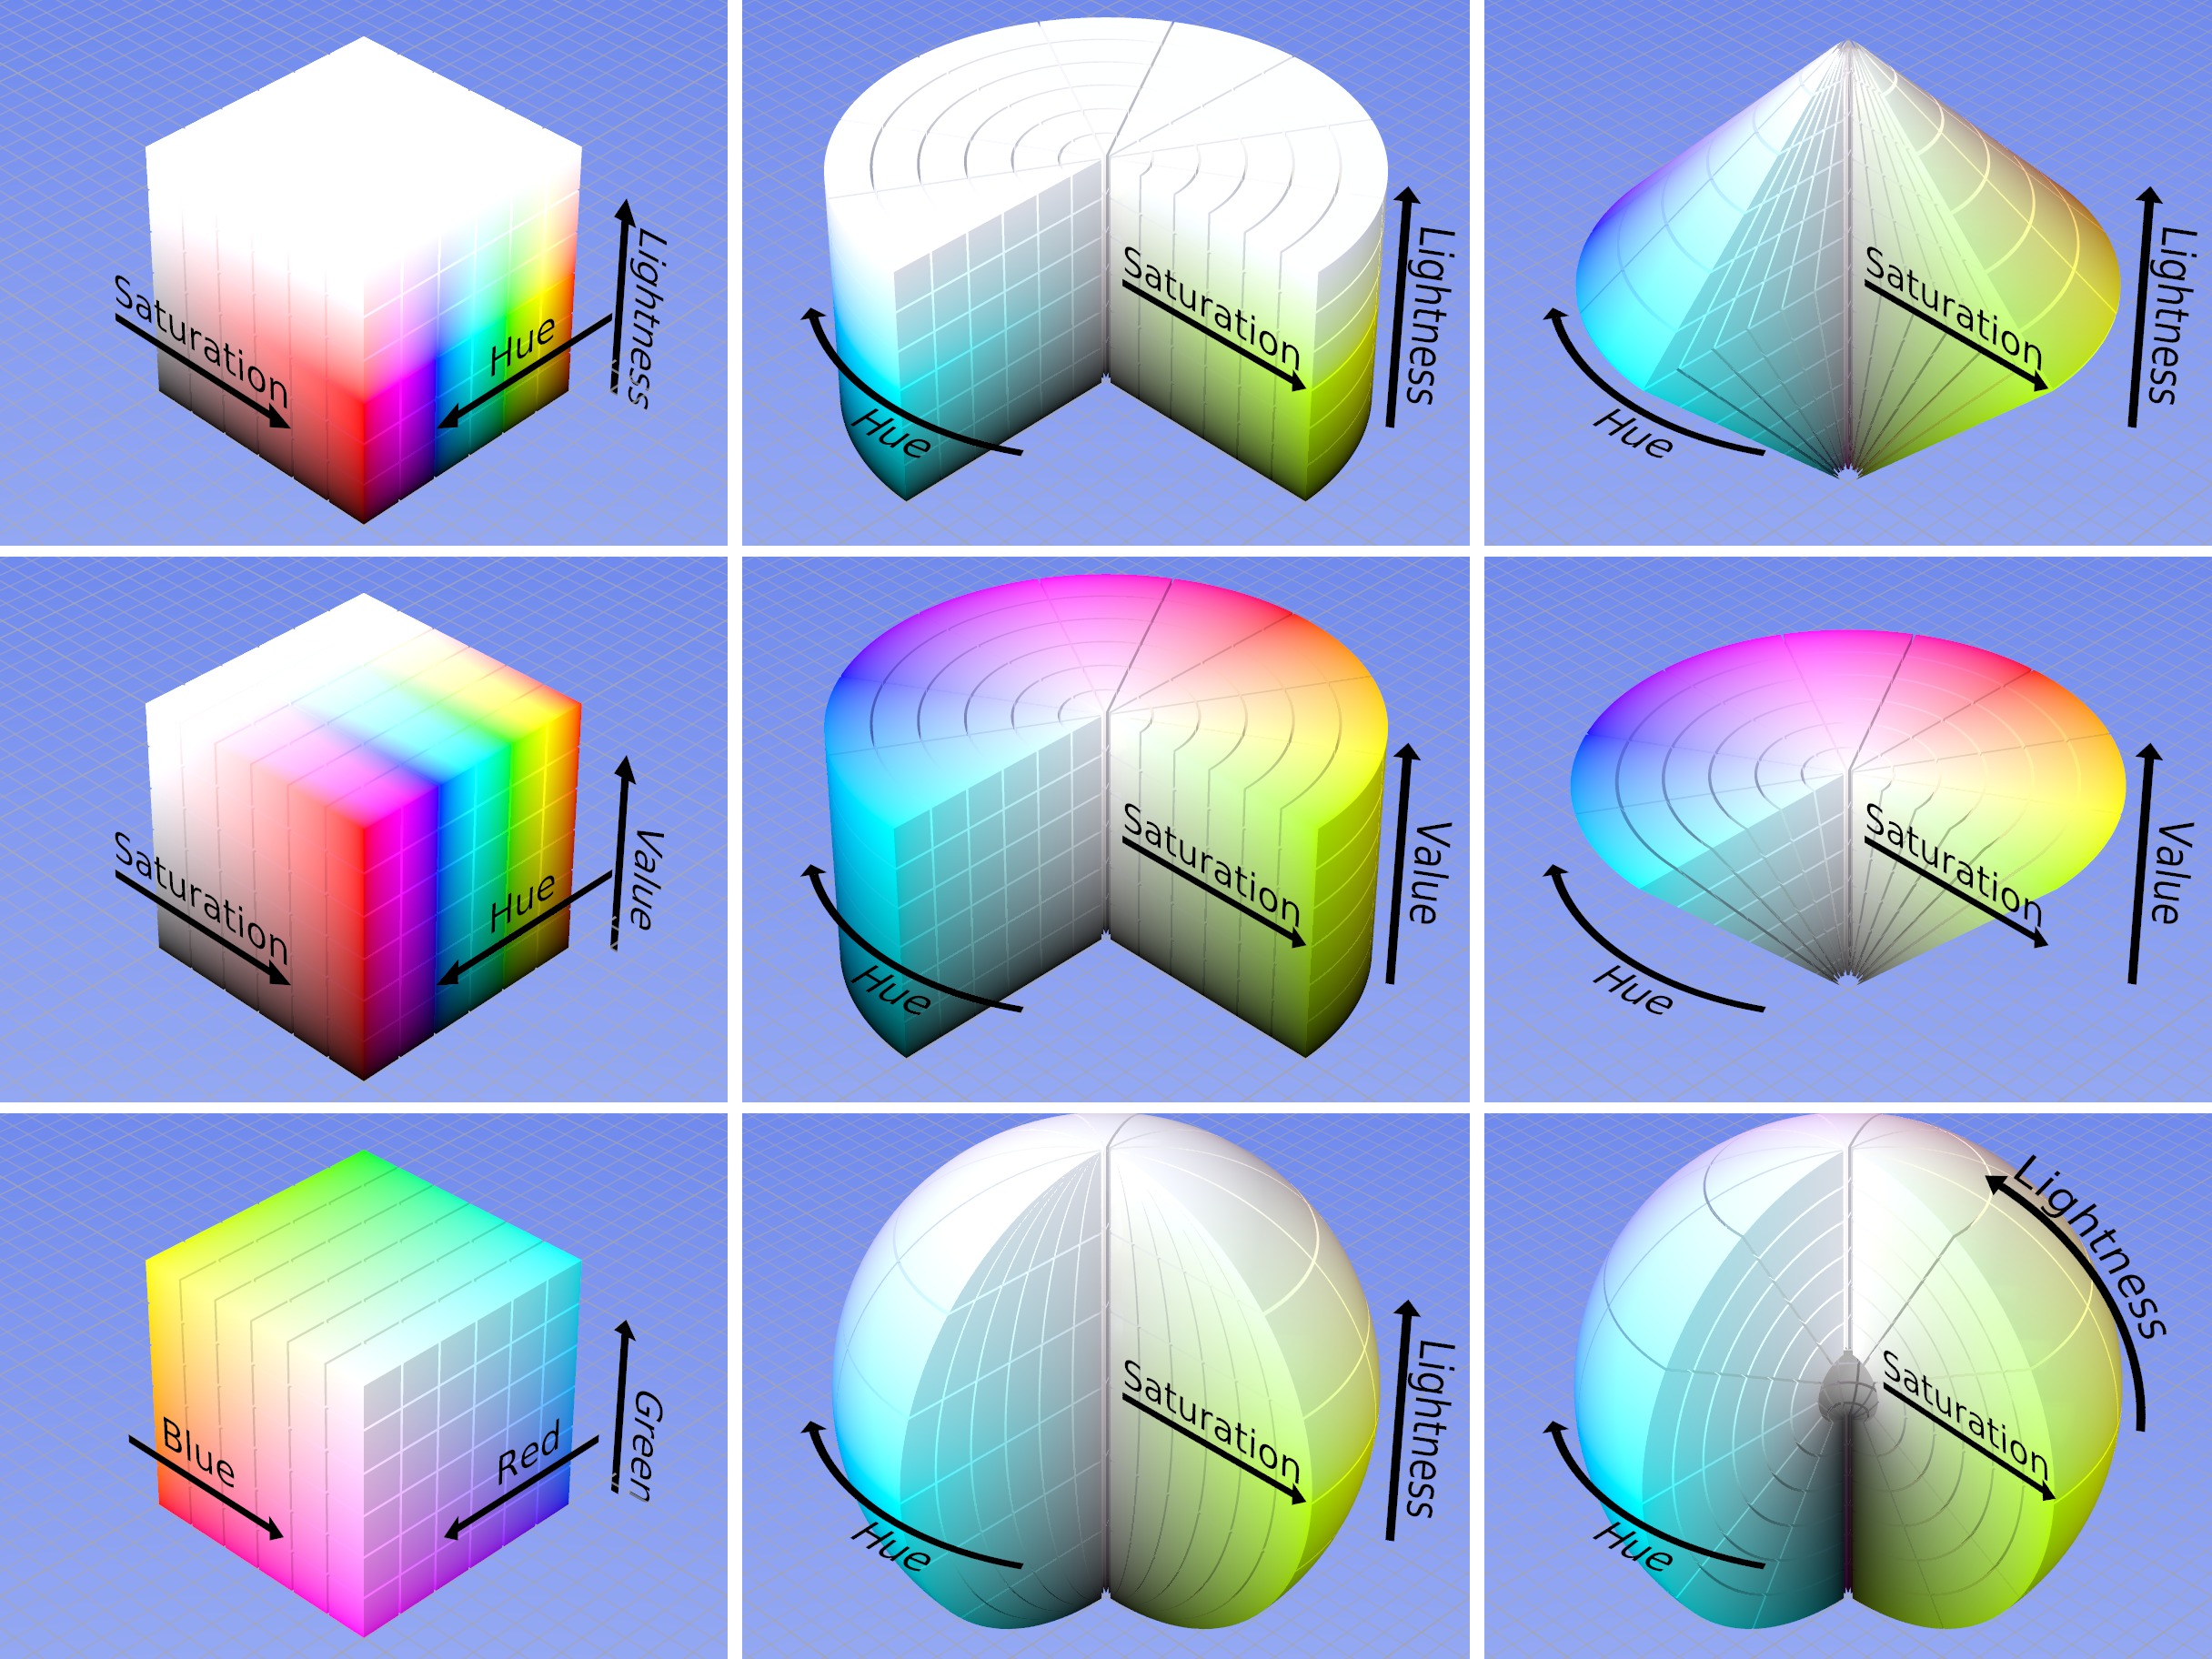
\includegraphics[height=.8\textheight]{figs/hsvrgb.png}
\end{center}
\end{frame}

\begin{frame}{Conversion entre systèmes de couleurs}
\begin{center}
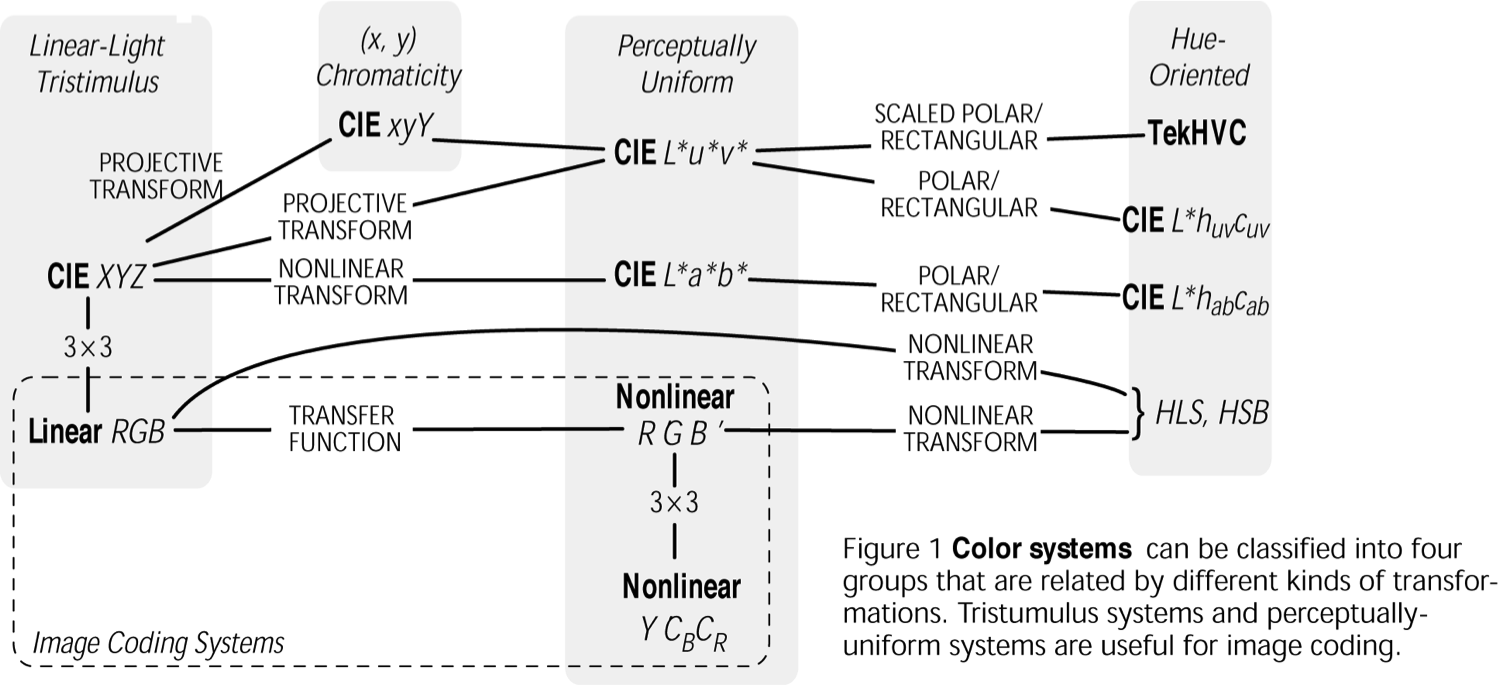
\includegraphics[height=.6\textheight]{figs/convcoul.png}
\end{center}
\end{frame}
